\section{Recovering An HDR Image and the Response Function}\label{sec:hdr}

The algorithm that has been used was the one found in \cite{rbs99}. In that
paper, the response function is initially assumed to be linear. This, while
already producing decent results, is of coruse not perfectly accurate for any
real camera. For this reason, \cite{rbs99} use an algorithm that iteratively
finds a good approximation of the response curve of the camera that has been
used as well as a high dynamic range image of the scene.

One problem I had was that, while the proposed weight function in \cite{rbs99}
sets the weight of extreme pixel values, i.~e. close to 0 or close to 255, very
low, they are still not zero, the weight for a pixel value of 255, for example,
is roughly 0.0183, cf. equation (5) in \cite{rbs99}. This results in absurd
looking images and response functions. An example is provided in figure~
\ref{fig:wrongweights}. The reason for this is probably that the denominator in
equation (8) becomes very small for high pixel values, especially because
images with longer exposure times are weighted more stongly, and those are more
likely to be overexposed.

\begin{figure}[h]
  \centering
  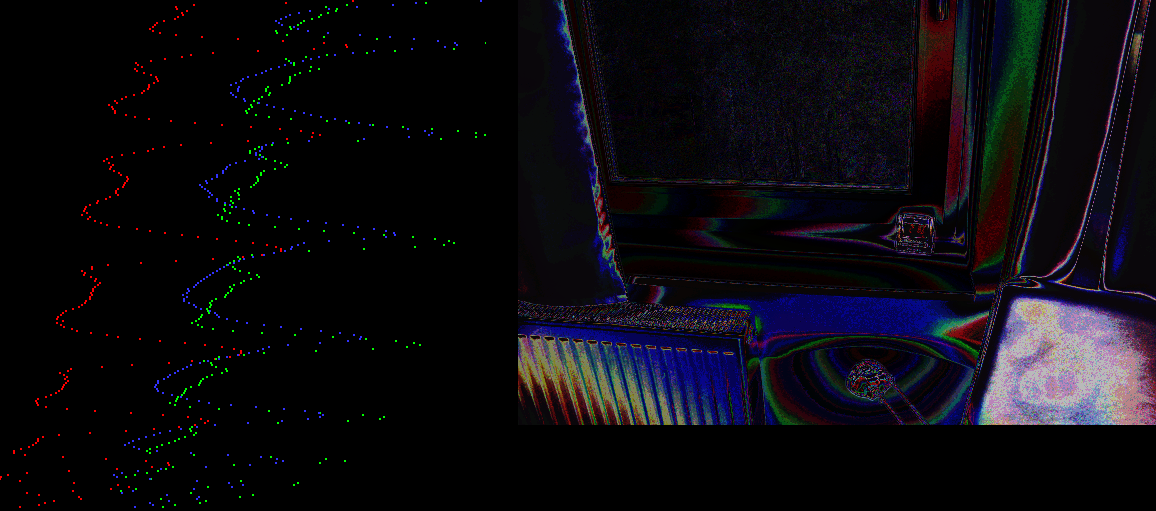
\includegraphics[width=\textwidth]{wrongweights.png}
  \caption{The image that results when the weights are not correct. For the
  response function on the left, the intensity goes up towards the right, and
  the resulting pixel value goes up towards the top. The intensity is on a
  logarithmic scale.}
  \label{fig:wrongweights}
\end{figure}

I had multiple test scenes, but the only other serious problems I encountered
happened in one where the camera was pointed directly at a lightbulb, leading
to parts of the image being completely overexposed even on the lowest exposure
setting. The first problem is that the denominator in equation (8) becomes 0 in
this case (because it was set to 0 due to the previously mentioned issue). The
numerator is also 0, which means the result is undefined. In subsequent
iterations, this quickly leads to all values of the response function being
undefined. This was fixed by setting the estimated luminance to 0 in these
cases.

This, however, is obviously not really correct - the pixels were completely
overexposed, and are now completely black in the final image. This can be fixed
by setting them to the maximum observed exposure value, since they are at least
that bright.

In figure \ref{fig:hdr} are two images that have been created by simulating a
certain exposure time after creating a high dynamic range image with this
algorithm, as well as the respective recovered response curves. The iterative
process was executed five times for these images.

\begin{figure}[h]
  \centering
  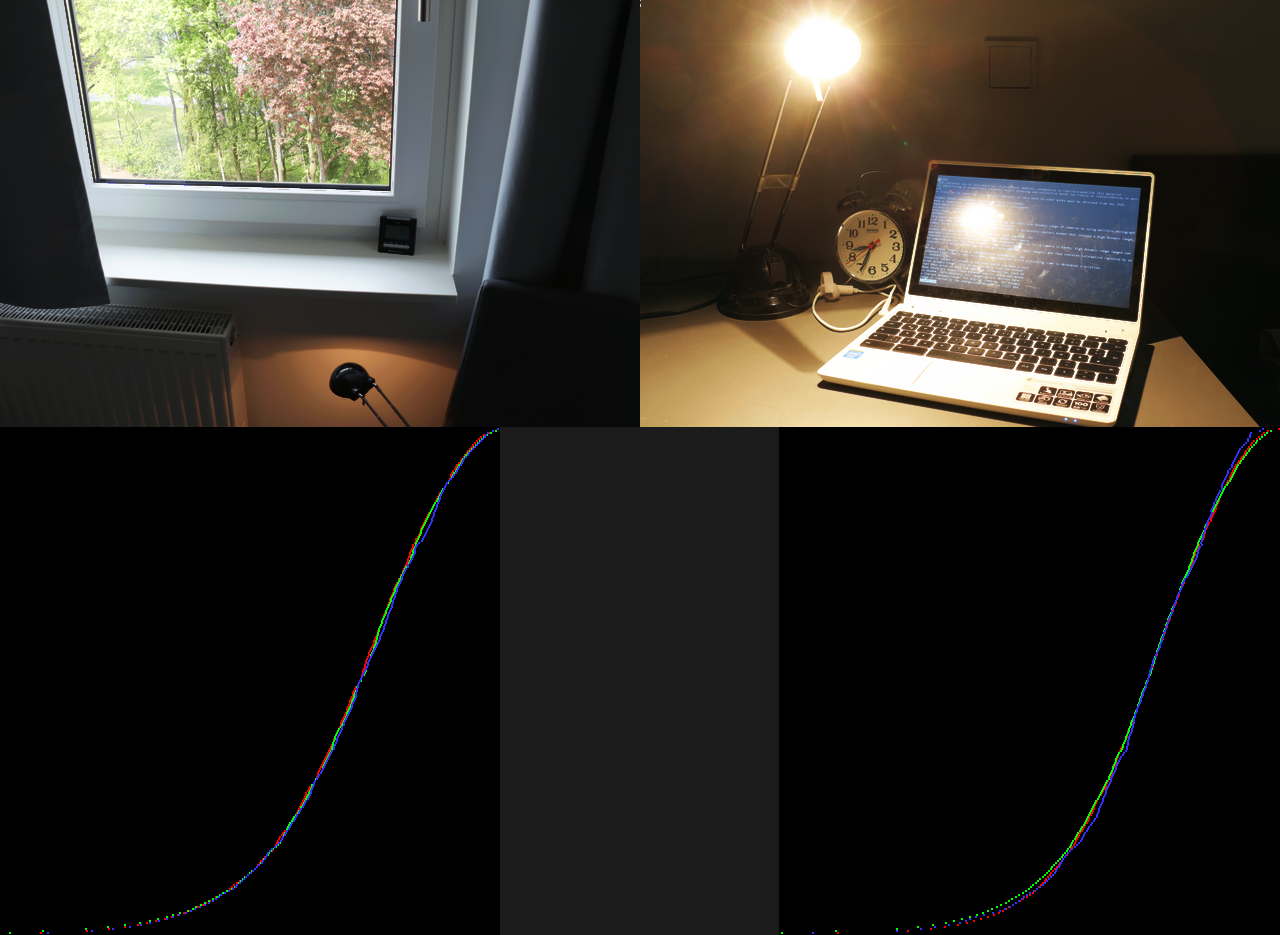
\includegraphics[width=\textwidth]{hdr.png}
  \caption{A window scene on the left, with simulated 1/100s exposure time, and
  an indoor scene on the right, looking at a lightbulb, with simulated 1/3s
  exposure time. Especially the blue response function appears to be slightly
  different for the images.}
  \label{fig:hdr}
\end{figure}
